\documentclass{article}
\usepackage{geometry}
\geometry{a4paper, top=3cm, bottom=3cm, left=3.5cm, right=3.5cm, heightrounded, bindingoffset=5mm}

%\documentclass[12pt, letterpaper, twoside]{article}
\usepackage[italian]{babel}
\usepackage[utf8]{inputenc}




\renewcommand{\contentsname}{Indice}

\usepackage{algorithm,algpseudocode}
\usepackage{hyperref}
\usepackage{amsmath}
\usepackage{caption}
\usepackage{float}
\usepackage{enumitem}
\hypersetup{hidelinks}
%\usepackage{authblk}


\newcommand{\code}[1]{\texttt{\detokenize{#1}}}

\usepackage{graphicx}
\graphicspath{ {./images/}  {../../test/} }

\title{
  Interactive Foreground Extraction using OpenCV and GrabCut Algorithm \\
  \large Tesina di Intelligenza Artificiale}


%\maketitle

%\title{\textbf{Tesina Intelligenza Artificiale}}
%\author[1] {Manuel Granchelli}
%\affil[1]{Dipartimento di Ingegneria Informatica, Università degli Studi Roma Tre}
\date{}

\begin{document}
\maketitle

\begin{flushleft}
\textbf{Manuel Granchelli} 
\hfill {\href{mailto:man.granchelli@stud.uniroma3.it}{\textbf{man.granchelli@stud.uniroma3.it}}} \\
\textit{Matricola: 512406}\\
\textit{Dipartimento di Ingegneria Informatica}\\
\textit{Università degli Studi Roma Tre}\\
\par\bigskip
\textbf{Repo GitHub:} \href{https://github.com/mgranchelli/foreground-extraction}{https://github.com/mgranchelli/foreground-extraction}
\end{flushleft}

\section*{Introduzione}
In questo documento verrà illustrata la foreground extraction interattiva attraverso l'utilizzo della libreria OpenCV e dell'algoritmo GrabCut. Il progetto è stato svolto implementando uno script Python. L'estrazione in primo piano avviene disegnando un rettangolo che contiene la regione da estrarre. Un esempio potrebbe essere quello di estrarre il volto di una persona da un'immagine, in questo caso il rettangolo dovrà includere al suo interno il volto. Nello script Python è stata definita una classe che permette di disegnare un rettangolo con il mouse e una volta disegnato il rettangolo viene richiamato l'algoritmo GrabCut presente all'interno della libreria OpenCV che restituisce in output una nuova immagine contenente la regione in primo piano all'interno del rettangolo disegnato. 

Open CV è una libreria open source per la visione artificiale e l'apprendimento automatico e GrabCut è un metodo di segmentazione delle immagini basato sui tagli dei grafi che non fa uso di tecniche di Machine Learning. Nella Computer Vision la segmentazione è una delle elaborazioni delle immagini cha avviene a livello intermedio.

Sono stati effettuati dei test su alcune immagini scaricate dal web. Lo script è stato lanciato su ogni immagine e per ogni immagine è stata evidenziata con un rettangolo la regione in primo piano da estrarre. 

\thispagestyle{empty}

\newpage

\tableofcontents
%\addcontentsline{toc}{section}{Unnumbered Section}

% Remove number page and start sections from this page
\thispagestyle{empty}

\clearpage
\pagenumbering{arabic}


\section{Introduzione alla Computer Vision}
La Visione Artificiale (Visione Computazionale, Computer Vision (CV)) è la disciplina che studia
modelli e metodi per abilitare le macchine alla comprensione e interpretazione delle informazioni visuali presenti in immagini fisse o in sequenze video. 
Un esempio di sistema di Computer Vision è il seguente: un computer elabora immagini di una scena reale, catturate da una o più (tele)camere, ed estrae da esse informazioni al fine di assumere decisioni in maniera automatica o semiautomatica.
Le informazioni estratte possono essere anche utilizzate per eseguire un'interpretazione 3D della scena.

\begin{flushleft}
La Computer Vision opera su due livelli:
\end{flushleft}

\begin{itemize}[noitemsep]
 \item A \textbf{basso livello} dove vengono eseguite, ad esempio, l'estrazione di primitive geometriche, forma, profondità, dimensione.
 \item Ad \textbf{alto livello} nel quale vengono eseguite operazione come, estrazione di proprietà delle forme, riconoscimento e classificazione di oggetti.
\end{itemize}
La risoluzione di molte problematiche di Computer Vision parte dall’analisi del processo di formazione dell’immagine di una scena. Le immagini vengono catturate da una scena 3D, solitamente, da una camera con lenti. Per poter proiettare i punti della scena 3D sul piano di immagine vengono utilizzati i due insiemi di \textbf{parametri di una camera reale} e \textbf{le equazioni fondamentali della proiezione prospettica}. I parametri della camera possono essere ottenuti tramite \textbf{calibrazione} della camera.
Successivamente le immagini sono \textbf{elaborate a basso livello}, dove viene eseguito lo smoothing che, a causa di errori casuali di misurazione e/o fallimenti del sistema, serve ad elaborare l'immagine e predire il valore di un pixel, dati quelli che lo circondano. In seguito, viene eseguito il rilevamento dei bordi che esegue un’astrazione dell’immagine originale (che è complessa e occupa diversi MB) verso una rappresentazione più compatta e astratta. I bordi, inoltre, possono corrispondere a importanti separazioni tra oggetti nella scena. Dopo l'elaborazione a basso livello vengono eseguite le \textbf{elaborazioni a livello intermedio} e tra queste troviamo la \textbf{segmentazione}.

La segmentazione opera a livello di immagine e non di scena ed è il processo di suddivisione di una immagine in gruppi sulla base della somiglianza dei pixel che li compongono.
L'idea alla base della segmentazione è quella di associare a ogni pixel determinate proprietà visive, come luminosità, colore e texture. All’interno di un oggetto, o di una sua singola parte, queste caratteristiche variano relativamente poco, mentre al confine tra un oggetto e un altro si può riscontrare un cambiamento significativo di almeno uno di questi attributi.
Lo scopo, quindi, è quello di suddividere l’immagine in insiemi di pixel in modo da soddisfare il più possibile questi vincoli.


Nel seguente progetto è stato utilizzato l'algoritmo GrabCut, che è un metodo di segmentazione delle immagini basato sui tagli dei grafi, dalla libreria OpenCV.

\section{OpenCV}
OpenCV (Open Source Computer Vision Library) è una libreria di software open source per la visione artificiale e l'apprendimento automatico. OpenCV è stato creato per fornire un'infrastruttura comune per le applicazioni di visione artificiale.
La libreria dispone di oltre 2500 algoritmi ottimizzati, che include un set completo di algoritmi di computer vision e machine learning sia classici che allo stato dell'arte. Questi algoritmi possono essere utilizzati per rilevare e riconoscere volti, identificare oggetti, classificare azioni umane nei video, tenere traccia dei movimenti della telecamera, tracciare oggetti in movimento, estrarre modelli 3D di oggetti, produrre nuvole di punti 3D da telecamere stereo, unire immagini per produrre un'alta risoluzione immagine di un'intera scena, trovare immagini simili da un database di immagini, rimuovere gli occhi rossi dalle immagini scattate con il flash, seguire i movimenti degli occhi e tanto altro.
OpenCV ha interfacce C++, Python, Java e MATLAB e nel seguente caso è stato utilizzato Python.


In particolare è stato utilizzato l'algoritmo GrabCut. Per poter utilizzare l'algoritmo occorre importare la libreria OpenCV e richiamare la funzione \code{grabCut()}.


\section{GrabCut Algorithm}
L'algoritmo GrabCut è stato progettato da Carsten Rother, Vladimir Kolmogorov e Andrew Blake di Microsoft Research Cambridge, UK. Si tratta di un algoritmo per l'estrazione in primo piano con un'interazione minima dell'utente.

Infatti, l'utente disegna un rettangolo nell'immagine intorno alla regione in primo piano e l'algoritmo lo segmenta in modo iterativo per ottenere il risultato. 
Nel seguente caso è stata creata una classe \textbf{BoundingBoxWidget} che permette all'utente di disegnare il rettangolo attorno alla regione. Una volta che l'utente ha disegnato il rettangolo viene richiamata la funzione \code{grabcut_algorithm}. Tale funzione prende in input l'immagine originale e le coordinate e dimensioni del rettangolo disegnato. La funzione inizializza una maschera nella quale vengono indicate le aree di probabile sfondo o primo piano, le coordinate e le dimensioni del rettangolo e due array \code{np.float64} di zeri di dimensione (1,65). Successivamente viene richiamata la funzione \code{grabCut()}, alla quale vengono passate le variabili inizializzate precedentemente, un intero che rappresenta il numero di iterazioni che farà l'algoritmo e il modo in cui viene generata l'area che contiene l'immagine in primo piano, in questo caso è stato disegnato un rettangolo, quindi come ultimo parametro della funzione è stato passato il parametro \textbf{cv.GC\_INIT\_WITH\_RECT}.
Infine, la funzione \code{grabcut_algorithm} genera e mostra una nuova immagine contenente la regione in primo piano all'interno del rettangolo disegnato.


\medbreak
Entrando nel dettaglio della funzione \code{grabCut()}, tutto ciò che è al di fuori del rettangolo disegnato viene considerato come sfondo. La funzione esegue un'etichettatura iniziale in base ai dati che vengono forniti in input ed etichetta i pixel che formano il primo piano e che formano lo sfondo.
Viene utilizzato un Gaussian Mixture Model (GMM) per modellare il primo piano e lo sfondo. In base ai dati che vengono forniti, il GMM crea una nuova distribuzione di pixel. I pixel sconosciuti sono etichettati come probabile primo piano o probabile sfondo, a seconda della loro relazione con gli altri pixel etichettati in precedenza in termini di statistiche sul colore (viene eseguito un raggruppamento).
Successivamente dalla distribuzione dei pixel viene generato un grafo. I nodi del grafo sono pixel. Vengono aggiunti due nodi, il \textbf{Source Node} e il \textbf{Sink node}. Ogni pixel in primo piano è connesso al Source Node e ogni pixel di sfondo è connesso al Sink node.
I pesi degli archi che collegano i pixel al Source Node/Sink node sono definiti dalla probabilità che un pixel sia in primo piano/sfondo. I pesi tra i pixel sono definiti dalle informazioni sugli archi o dalla somiglianza dei pixel. Se c'è una grande differenza nel colore dei pixel, l'arco tra di loro avrà un peso ridotto.
Infine, viene utilizzato un algoritmo \textit{mincut} per segmentare il grafo. Il grafo viene tagliato in due separando il nodo sorgente e il nodo sink con una funzione di costo minimo. Tale funzione è pari alla somma di tutti i pesi degli archi tagliati. Dopo il taglio, tutti i pixel collegati al Source Node diventano pixel in primo piano e quelli collegati al Sink node diventano pixel di sfondo.
Nella Figura \ref{fig:graph-cut} è rappresentato il processo dall'input all'immagine segmentata.

\begin{figure}[H]
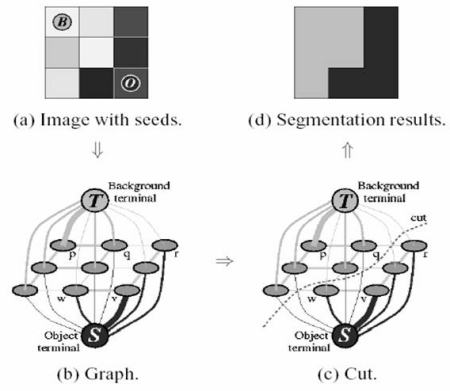
\includegraphics[scale=0.5]{graph-cut}
\centering
\captionof{figure}{Graph cut}
\label{fig:graph-cut}
\end{figure}

\section{Test e Risultati}
I test sono stati eseguiti con alcune immagini scaricate dal web. Per ogni immagine è stato lanciato lo script Python nel seguente modo: \code{python3 foreground-extraction.py -i path-image}, \code{path-image} è il percorso dell'immagine da processare, se non specificato viene caricata l'immagine di default \textit{avengers.jpg} presente all'interno del repo nella cartella \href{https://github.com/mgranchelli/foreground-extraction/assets/images}{\textit{assets/images}}.

Una volta caricata l'immagine è stato disegnato con il mouse il rettangolo sulla regione da estrarre e lo script restituisce il risultato. 
\begin{flushleft}
In seguito, è possibile osservare alcuni test effettuati.
\end{flushleft}


\begin{figure}[H]
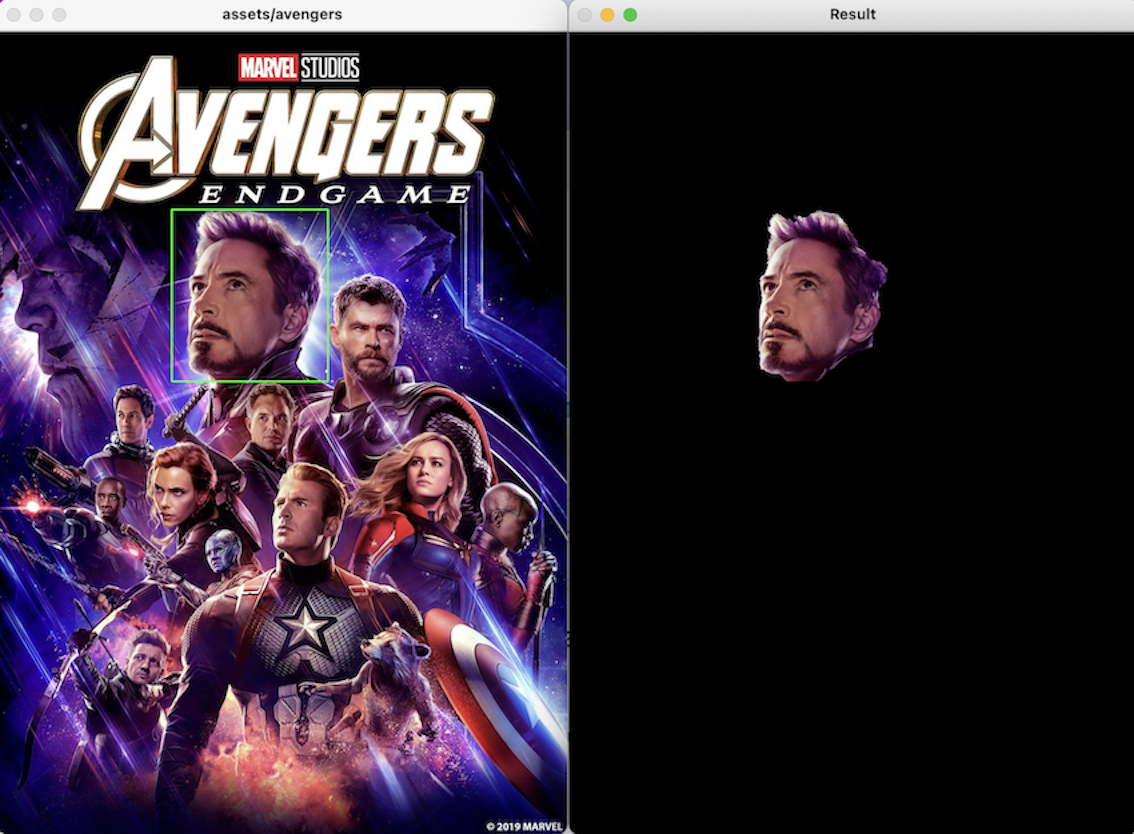
\includegraphics[scale=0.5]{test-avengers-1}
\centering
\captionof{figure}{Test 1}
\label{fig:test1}
\end{figure}

\begin{figure}[H]
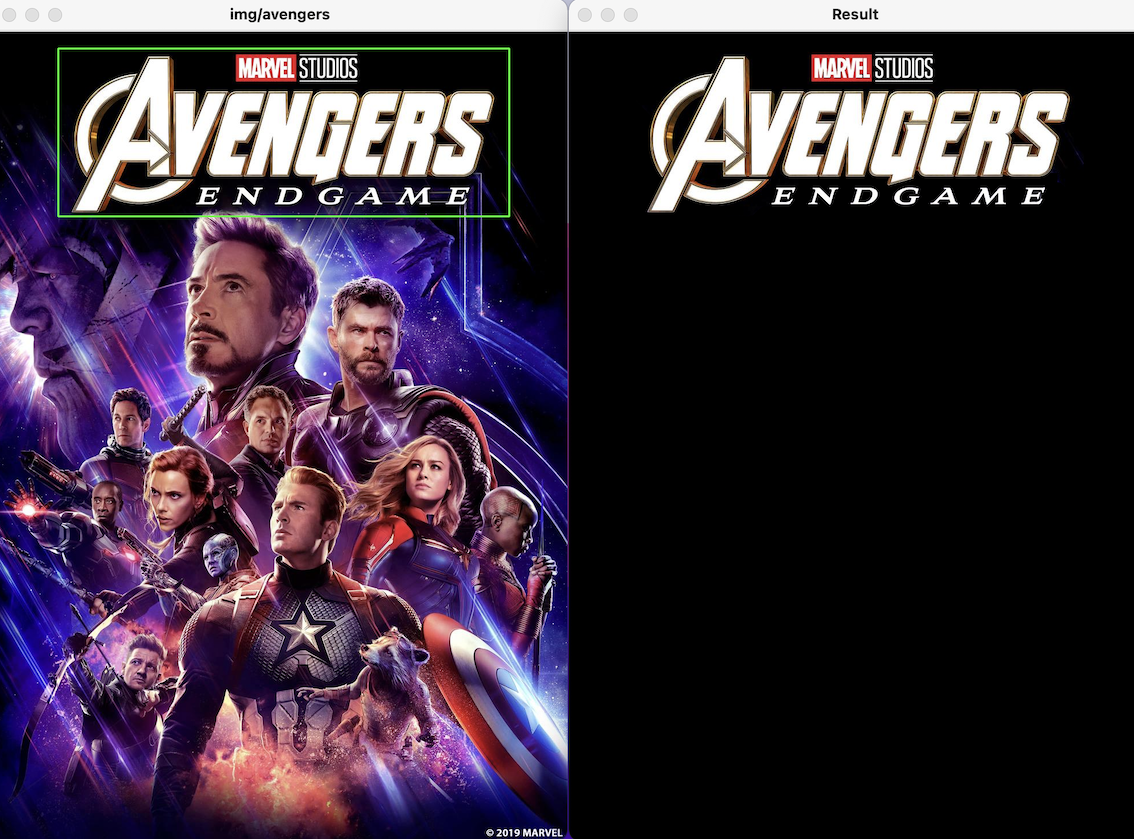
\includegraphics[scale=0.5]{test-avengers-2}
\centering
\captionof{figure}{Test 2}
\label{fig:test2}
\end{figure}


\begin{figure}[H]
\centering
\begin{minipage}{.5\textwidth}
  \centering
  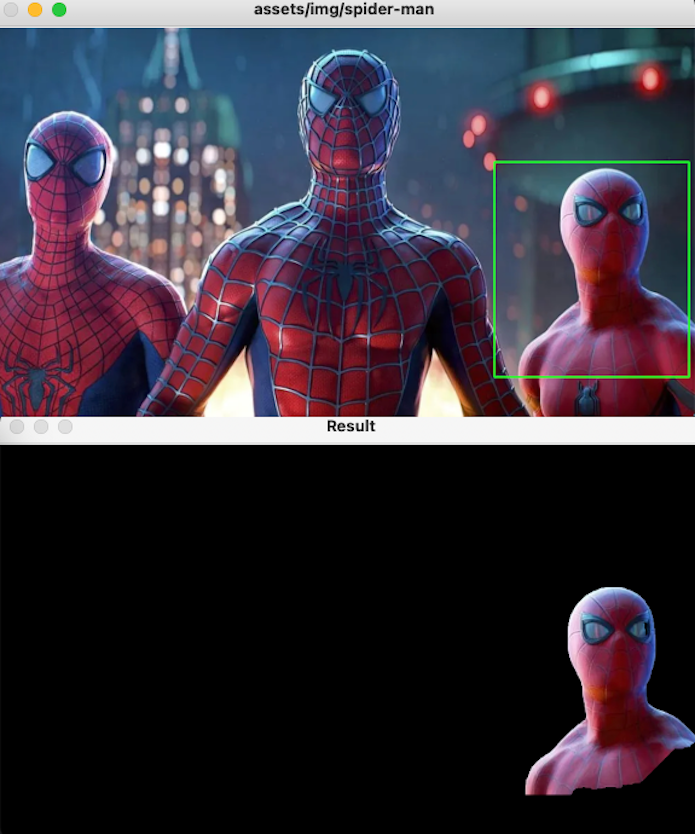
\includegraphics[scale=0.27]{test-spider-man}
  \captionof{figure}{Test 3}
  \label{fig:test3}
\end{minipage}%
\begin{minipage}{.5\textwidth}
  \centering
  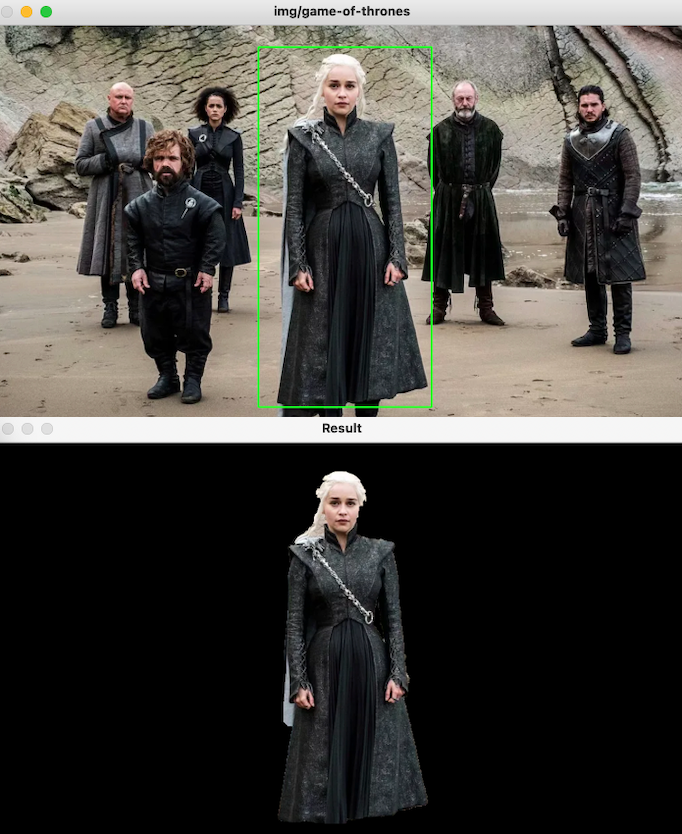
\includegraphics[scale=0.27]{test-game-of-thrones}
  \captionof{figure}{Test 4}
  \label{fig:test4}
\end{minipage}
\end{figure}


\begin{figure}[H]
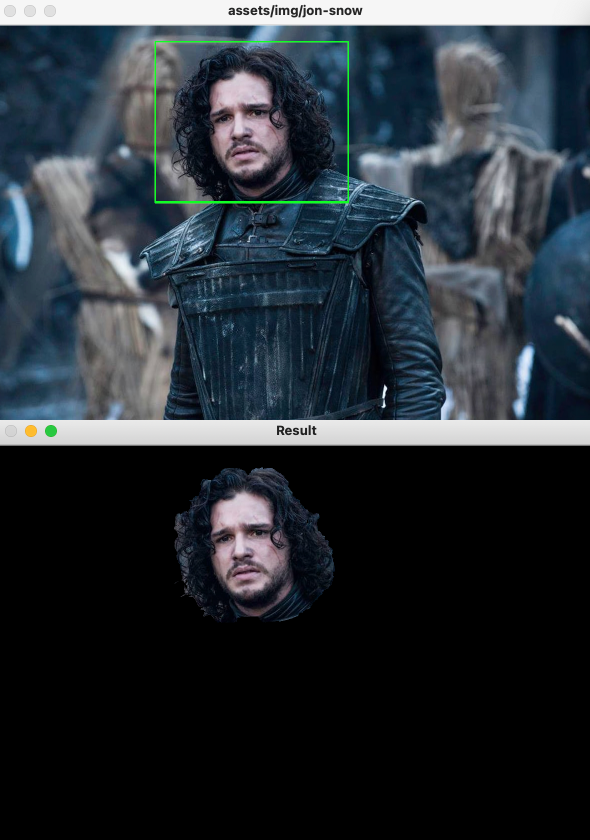
\includegraphics[scale=0.35]{test-jon-snow}
\centering
\captionof{figure}{Test 5}
\label{fig:test5}
\end{figure}

Dai risultati si è osservato che in alcuni casi, la segmentazione non viene eseguita correttamente, ad esempio, l'algoritmo potrebbe contrassegnare una parte della regione in primo piano come sfondo. 
Come si può osservare dal risultato del Test 4 (Figure \ref{fig:test4}) parte dei capelli vengono tagliati.
In questo caso, l'utente potrebbe ritoccare manualmente con tratti bianchi le parti della regione che devono essere ottenute in primo piano come risultato e con tratti neri le parti che formano lo sfondo. 
I ritocchi possono essere fatti creando una nuova un'immagine contenente i tratti bianchi e/o neri e la nuova immagine verrà utilizzata dall'algoritmo GrabCut come ulteriore maschera per poter identificare meglio la regione in primo piano. L'implementazione di questa funzione è disponibile nella \href{https://docs.opencv.org/3.4/d8/d83/tutorial_py_grabcut.html}{\textit{documentazione}} di OpenCV e nel seguente progetto non è stata inserita.



\end{document}